\section{Proposed timeline}

I have outlined a substantial amount of work of be done in this proposal. %you probably realized while reading through the chapters, I have proposed a substantial amount of work. 
The three proposed chapters require huge amounts of time just to generate the data, which is compounded by analysis and writing. 
I have attempted to trim the fat where possible, reducing the amount of computation needed for each chapter. 
Even still, my current plan is to defend late next spring.
To have any hope of meeting that deadline, I need a plan. 
Therefore, I present my timeline for when I will perform the various tasks for each chapter Figure \ref{fig:timeline}. %, with some extra about the time required for each task. 

% Go into more detail on how the brains work? Encoding?
\begin{figure}[h!]
    \centering
    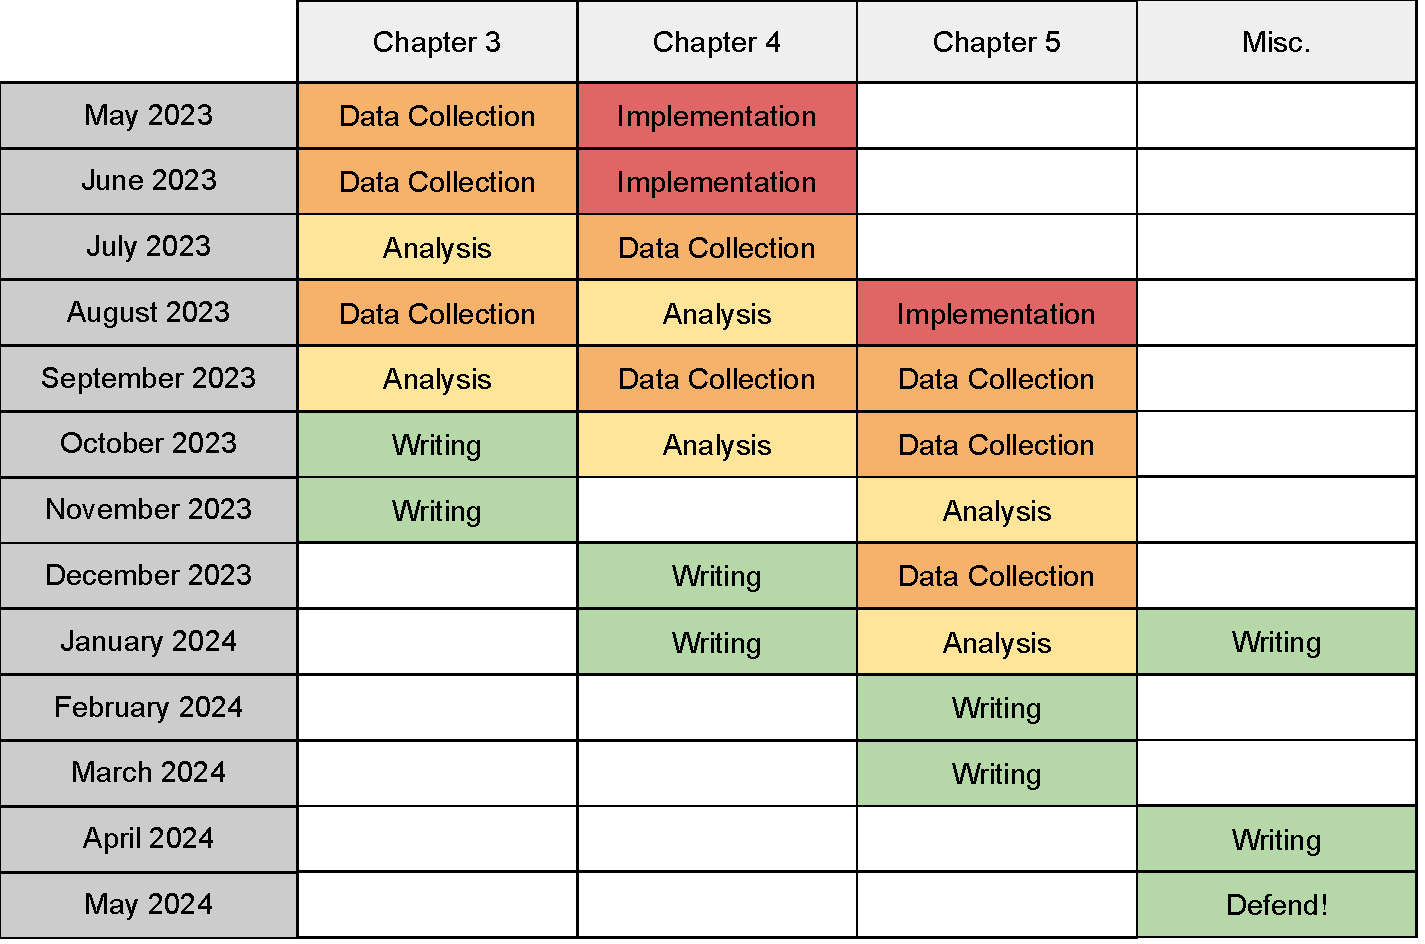
\includegraphics[width=0.95\textwidth]{08_timeline/media/timeline.pdf}
    \caption{My proposed timeline for completing the proposed chapters and my dissertation as a whole. 
    The miscellaneous column includes writing the introduction and conclusion of the dissertation.
    Remainder of explanation in text.}
    \label{fig:timeline}
\end{figure}


As stated above, all three proposed chapters, but especially Chapters \ref{chap:replaying_associative_learning} and \ref{chap:varying_environments}, are very computationally expensive. Thus I have included two initial months of data collection for both, with an extra month allotted for any additional data collection that was identified as needed during analysis. 
The other chapter, Chapter \ref{chap:simplified_model}, will deal with an enormous amount of data, but the bitstring model makes that data much faster to collect. 
As such, it receives only one month of initial data collection and one month for collecting any additional data. 
%It should be noted that once the pipeline for collecting data is in place, collecting data is mostly a hands off process, allowing me to perform other tasks at the same time.
%I have created infrastructure to allow thousands of jobs to queue and run on the HPCC with no human oversight needed. 

Chapter \ref{chap:replaying_associative_learning} is not allotted any dedicated implementation time, as all the pieces are in place thanks to Chapter \ref{chap:alife_submission}.
This chapter is ready to begin data collection once the comprehensive examination has concluded.
Chapter \ref{chap:simplified_model} is allotted a very conservative two months of implementation, as all the pieces (NK landscapes, enumeration and replay pipelines) exist and will only require tweaks and testing. 
Finally, all the environments and Avida changes are already implemented in MABE2, and thus Chapter \ref{chap:varying_environments} is given a single month of dedicated implementation time to connect the pieces together. 

Each project is given two months for analysis, one after the initial data collection and one more after any additional data collection is completed. 
%Note that once the analyses have been created, I will be running many of these analyses as soon as the data is finished and pulled from the HPCC. 
%As such, I will often be performing other tasks, such as writing or implementing, during the months marked as analysis. 

Finally, all of these projects will need to be written up. %, and writing is the hardest for me to judge the time required. 
As things stand, I have allotted two months of writing time for each proposed chapter. 
I have also allotted two months to writing the other pieces of the dissertation (e.g., introduction, conclusion, and any needed appendices). 

Fortunately, data collection is mostly hands-off once it has been started, and most analyses will be reused for the various projects, saving substantial time in the long run. 
%It is not shown, but I will also be drafting the early parts of each chapter (e.g., the introduction and methods) as I collect data and analyze the data. 
Having different projects going simultaneously is my preferred way to work, as I often switch between them when I hit a rut, allowing me to come back later with a fresh mind. 
As such, I have attempted to structure this timeline such that I always have one active task (coding or writing) occurring concurrently with data collection and analysis. 
While I could not easily show it in the figure, I will begin writing the introduction and methods to each chapter during the early data collection and analysis phases. 

While it will be a ton of work, I look forward to it. 
%I have tried to structure this timeline in a way that I am often collecting data for one project while doing writing, coding, or analyzing one or two other chapters, as data collection does not require much active effort in these systems. 


% Mention that I will be TAing in the fall but not the spring?